\chapter{Funciones de Distancia con Signo}
\section{Introducción}
Hemos presentado anteriomente las funciones de distancia con signo como definición matemática, pero ahora debemos cuestionarnos, ¿Cómo podemos definir funciones de distancia con signo propias?, ¿Qué operadores existen?

%https://www.iquilezles.org/www/articles/distfunctions/distfunctions.htm
\begin{definition}
Una función de distancia con signo, se dice exacta si está definido sobre la métrica euclídea.
\end{definition}

Vamos a definir algunas \textit{funciones de distancia con signo} \textbf{primitivas} sobre \(\mathbb{R}^2\) y posteriormente sobre \(\mathbb{R}^3\). Las definiremos centradas en el \((0,0)\) y en el \((0,0,0)\), respectivamente. Que posteriormente podremos trasladarlo o rotarlo utilizando operadores.
%https://www.iquilezles.org/www/articles/distfunctions2d/distfunctions2d.htm
\section{Primitivas sobre \(\mathbb{R}^2\)}
Estas primitivas son fundamentales para finalmente contruir distintas funciones sobre \(\mathbb{R}^3\) ya que muchas de estas primitivas, son facilmente generalizables o se utilizan junto a un operador como extrusión o revolución figuras sobre.\\\\
Para visualizar estas funciones, vamos a hacer uso también de \textit{Shadertoy} y vamos a modificar levemente el código por defecto. Utilizaremos el color rojo para indicar el interior de la figura, el color azul para el exterior y el color blanco para indicar que está próximo a una isosuperficie, utilizando un valor empírico \(\epsilon=0,01\).
\begin{lstlisting}
#define EPSILON 0.01
void mainImage( out vec4 fragColor, in vec2 fragCoord )
{
    vec2 p = (fragCoord-iResolution.xy * 0.5)/min(iResolution.x, iResolution.y);
    // Aplicamos la funcion de distancia con signo sdf junto con los parámetros que lo definen.
    float d = ...;
    
    vec3 col;
    if(abs(d) < EPSILON){
        col = vec3(1.0);
    }else{
        if(d < 0.0){
    		col = vec3(1.0, 0., 0.);
    	}else{
    		col = vec3(0., 0., 1.0);
    	}
    	// Número de repeticiones.
        float k = 10.0;
        col = col * (0.5 + 0.5 * (fract(abs(d) * k)));
    }
    fragColor = vec4(col, 1.);
}
\end{lstlisting}

\subsection{Circunsferencia exacta}
La definición de esta figura es muy simple, la distancia desde cualquier punto \(\Vec{p}\) hasta \((0,0)\) está definido por el módulo del vector \(\vert\vert\Vec{p}\vert\vert\), esto crea una función de distancia positiva con un isoperímetro \(S=\{(0,0)\}\), si le restamos el radio \(r\), conseguiremos lo querido, anular aquellos puntos a distancia \(r\). Cuando el vector está en el interior de la circusnferencia (el módulo del vector es inferior al radio), \(\vert\vert\Vec{p}\vert\vert < r \longrightarrow \vert\vert\Vec{p}\vert\vert - r=d < 0\) siendo la distancia negativa o el interior de la figura. En caso de que el módulo del vector coincide con el radio, \(\vert\vert\Vec{p}\vert\vert = r \longrightarrow \vert\vert\Vec{p}\vert\vert - r=d = 0\), es decir, estamos sobre el isoperímetro. Mientras que si el módulo es mayor, \(\vert\vert\Vec{p}\vert\vert > r \longrightarrow \vert\vert\Vec{p}\vert\vert - r=d > 0\) la distancia será positiva en el exterior.
\begin{lstlisting}
// Circunsferencia Exacta
float SDFCircunsferencia(vec2 p, float r){
    return length(p) - r;
}
\end{lstlisting}
\begin{figure}[H]
  \centering
  \captionsetup{justification=centering}%,margin=2cm
  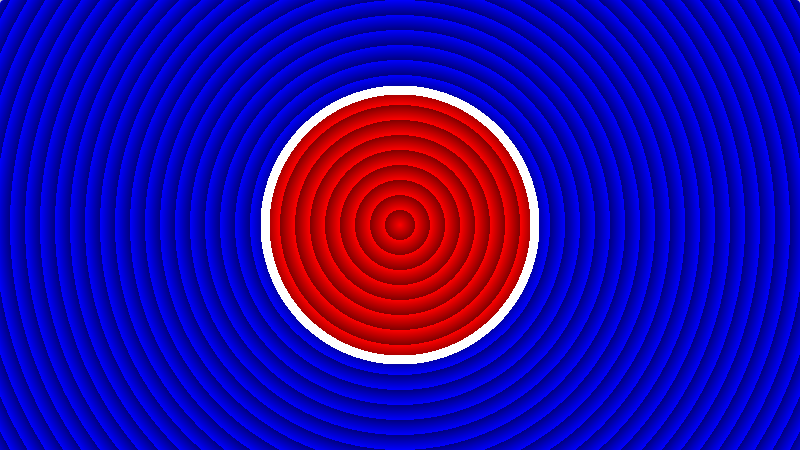
\includegraphics[width=0.8\textwidth]{secciones/imagenes/sdf/2d/sdf_circunsferencia.png}\label{fig:circ}
  \caption{Circunsferencia FDS radio \(0.3\)}
\end{figure}

\subsection{Rectángulo exacto}
Para calcular de forma exacta esta función vamos a definir algunos operadores sobre los vectores, que están definidos en GLSL.
\[\vert(x_0,x_1,\dots,x_n)\vert=(\vert x_0\vert,\vert x_1\vert,\dots,\vert x_n \vert)\]
\[\max\left((x_0,x_1,\dots,x_n), k\right)=(\max( x_0, k), \max(x_1, k),\dots, \max(x_n, k))\]
El operador valor absoluto es muy útil ya que, en caso de existir simetría axial en x e y, que lo hay, podemos reducir nuestro problema a un único cuadrante. Debemos tener en cuenta que la las medidas originales son reducidas a la mitad ya que solo estamos observando el primer cuadrante que representa \(\dfrac{1}{4}\) de la figura. Estas medidas son expresadas de manera vectorial tales que \[\Vec{s'}=(w', h')=\left(\dfrac{w}{2},\dfrac{h}{2}\right)=\dfrac{\Vec{s}}{2}\]
Una vez hecho esto, vamos a reducir el problema en 4 regiones.
\begin{figure}[H]
  \centering
  \captionsetup{justification=centering}%,margin=2cm
  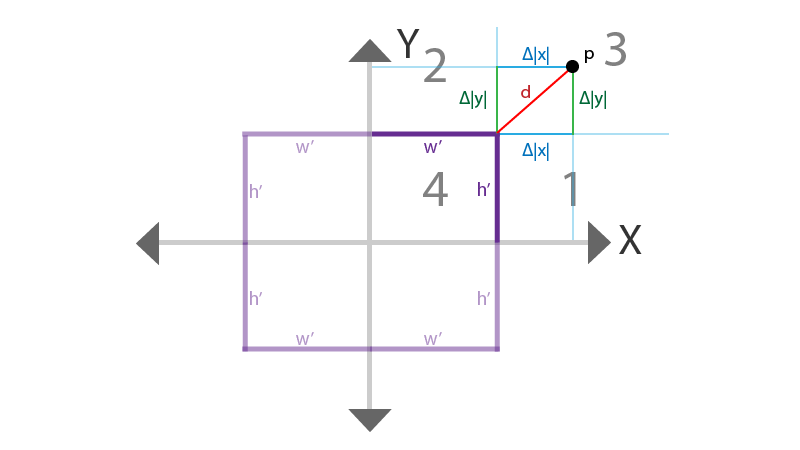
\includegraphics[width=1.0\textwidth]{secciones/imagenes/sdf/proofs/proof_rectangle.png}\label{fig:subproblem}
  \caption{División del rectángulo en 4 regiones o subproblemas.}
\end{figure}
Vamos a preservar la métrica euclídea suponiendo que se ha posicionado el punto \(\Vec{p}=\vert(x,y)\vert=(\vert x\vert, \vert y \vert)\) en cada una de las regiones.
\begin{enumerate}
    \item \textbf{Región 1}. Se trata de encontrar la distancia al lado derecho, esto es sencillo, bastaría con hacer \(\Delta x=\vert x\vert-w'\).
    \item \textbf{Región 2}. De manera similar al anterior, la distancia al lado superior, será \(\Delta y=\vert y\vert-h'\).
    \item \textbf{Región 3}. En esta región vamos a calcular la distancia a la esquina del rectángulo, \(\vert\vert \vert\Vec{p}\vert-\Vec{s'}\vert\vert = \sqrt{\left(\vert x\vert-w'\right)^2+\left(\vert y\vert-h'\right)^2}\).
    \item \textbf{Región 4}. Esta región puede considerarse la más difícil de calcular, debemos utilizar el mismo cálculo que el utilizado para los lados, pero nos quedaremos con la distancia máxima del cálculo, ya que esta es negativa, al estar en el interior de la figura. Deberá anularse la componente cuanto este cálculo sea positivo, es decir, esté en la \textbf{Región 1, 2}.
    \[argmax(\Vec{a})=min(max(\Vec{a}_x, \Vec{a}_y), 0)\]
    Por lo que la distancia interior, será \(argmax(\vert\Vec{p}\vert-\Vec{s'})\).
\end{enumerate}

Podríamos crear una función a trozos, definida mediante diferentes \textit{ifs} para cada una de las regiones, pero queremos que además de ser exacta, sea eficiente, por lo que vamos a mirar en que relación tienen las diferentes regiones según la posición del punto. Es importante observar que la \textbf{Región 3} contiene en su ecuación a las \textbf{Regiónes 1,2}, por lo que deben existir casos particulares. Cuando \(\Delta \vert x\vert =\vert x\vert-w'=0\longrightarrow \sqrt{\left(\vert y\vert-h'\right)^2} = \vert y\vert-h'=\Delta \vert y\vert\), que concuerda con la \textbf{Región 2} en la recta \(y=h'\) pero cuando \(\Delta \vert x\vert < 0\), vemos que la componente \(y\) no queda isolada, para que esto ocurra, haremos \(\max\left(\Delta \vert x\vert, 0\right)\), haciendo que la \textbf{Región 2 y 3} queden unificadas. De manera equivalente para la \textbf{Región 1 y 3}, tenemos \(\max\left(\Delta \vert y\vert, 0\right)\), esto hace que la ecuación unificada para las \textbf{Regiones 1, 2 y 3} sea la siguiente,
\[SDFRectangulo_{\Vec{s'}}(\Vec{p})\approx \vert\vert\max\left(\vert\Vec{p}\vert-\Vec{s'},0\right)\vert\vert\]
Finalmente, no es difícil observar que \(\Delta\vert x\vert=\Delta\vert y\vert=0\) cuando nos encontramos en la \textbf{Región 4}, por lo que bastará sumar la distancia de esta región para obtener la ecuación exacta.
\[SDFRectangulo_{\Vec{s'}}(\Vec{p})= \vert\vert\max\left(\vert\Vec{p}\vert-\Vec{s'},0\right)\vert\vert + argmax(\vert \Vec{p}\vert - {s'})\]
\begin{lstlisting}
// Rectángulo Exacto
float SDFRectangulo(vec2 p, vec2 s){
    vec2 a = abs(p) - s;
    return length(max(a, 0.0)) + min(max(a.x, a.y), 0.0);
}
\end{lstlisting}
\begin{figure}[H]
  \centering
  \captionsetup{justification=centering}%,margin=2cm
  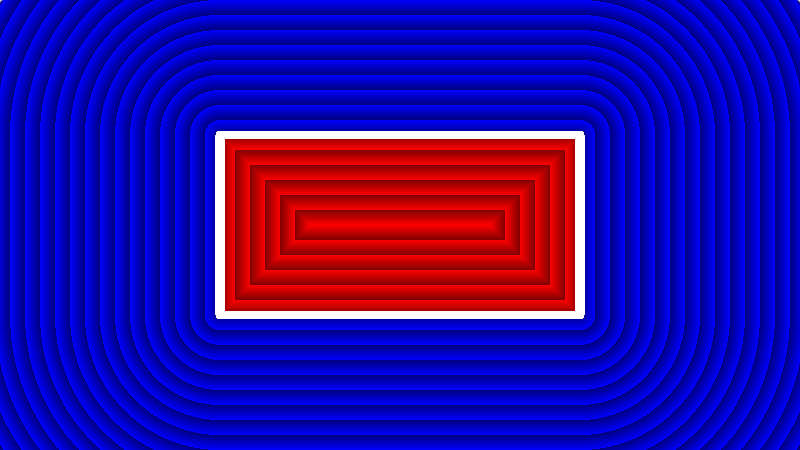
\includegraphics[width=0.8\textwidth]{secciones/imagenes/sdf/2d/sdf_rectangulo.png}\label{fig:rectaangulo}
  \caption{Rectángulo FDS de dimensiones \(\Vec{s'}=(0.4, 0.2)\)}
\end{figure}

\subsection{Recta exacta}
Veamos la distancia a una recta que pasa por dos puntos \(\Vec{a},\Vec{b}\). Pero antes, definimos la proyección escalar de \(\Vec{a}\) sobre \(\Vec{b}\) tal que:
\[ \text{proy}_{\Vec{b}}\Vec{a}=\left(\dfrac{\Vec{a}\cdot\Vec{b}}{\vert \Vec{b}\vert}\right)\dfrac{\Vec{b}}{\vert\Vec{b}\vert}=\left(\dfrac{\Vec{a}\cdot\Vec{b}}{\vert \Vec{b}\vert^2}\right)\Vec{b}=\left(\dfrac{\Vec{a}\cdot \Vec{b}}{\Vec{b}\cdot \Vec{b}}\right)\Vec{b}\]

\begin{figure}[H]
  \centering
  \captionsetup{justification=centering}%,margin=2cm
  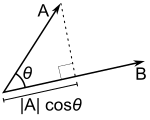
\includegraphics[width=0.3\textwidth]{secciones/imagenes/proyeccion.png}\label{fig:proyection}
  \caption{Proyeccinón \(\Vec{a}\) sobre \(\Vec{b}\)}
\end{figure}
Para aplicar esta ecuación, vamos a calcular los dos vectores, el vector de dirección \(\Vec{v}=\Vec{b}-\Vec{a}\) de la recta, que está centrado en el origen. Por otro lado, el vector a proyectar \(\Vec{w}=\Vec{p}-\Vec{a}\) que depende de la posición \(\Vec{p}\), centrado también en el origen. Definimos la función de distancia con signo, cómo:
\[SDFRecta_{\Vec{a},\Vec{b}}(\Vec{p})=\vert\vert (\Vec{p}-\Vec{a}) - \text{proy}_{\Vec{p}-\Vec{a}}\left(\Vec{b}-\Vec{a}\right)\vert\vert\]

\begin{lstlisting}
// Operador Proyección a sobre b
vec2 proy(in vec2 a, in vec2 b){
    return b * dot(b, a) / dot(b, b);
}
// Línea Exacto
float SDFRecta(vec2 p, vec2 a, vec2 b){
    vec2 v = p - a;
    vec2 w = b - a;
    return length(v -  proy(v, w));
}
\end{lstlisting}
\begin{figure}[H]
  \centering
  \captionsetup{justification=centering}%,margin=2cm
  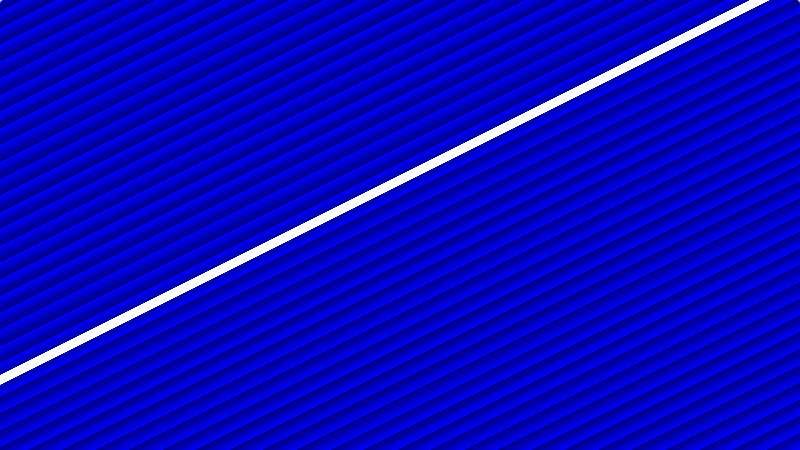
\includegraphics[width=0.8\textwidth]{secciones/imagenes/sdf/2d/sdf_recta.png}\label{fig:recta}
  \caption{FDS Recta que pasa por \(\Vec{a}=(0.2, 0.2), \Vec{b}=(0.0, 0.1)\)}
\end{figure}

\subsection{Segmento exacto}
Se trata de un caso particular del operador proyección entre dos vectores \(\Vec{a}, \Vec{b}\). 
\[ \text{proy}_{\Vec{b}}\Vec{a}=\left(\dfrac{\Vec{a}\cdot \Vec{b}}{\Vec{b}\cdot \Vec{b}}\right)\Vec{b}\]
Observamos que \(\dfrac{\Vec{a}\cdot \Vec{b}}{\Vec{b}\cdot \Vec{b}}\) es el factor de proyección que está en \(\mathbb{R}\). Cuando este es cero, la proyección será \((0,0)\) y cuando sea \(1\), tomará el vector \(\Vec{b}\). Solo tendremos que limitar este valor de este factor en el intervalor \([0,1]\):
\[ \text{proy[0,1]}_{\Vec{b}}\Vec{a}=\max\left(\min\left(\dfrac{\Vec{a}\cdot \Vec{b}}{\Vec{b}\cdot \Vec{b}}, 0\right), 1\right)\Vec{b}\]

\begin{lstlisting}
// Operador Proyección [0,1] a sobre b
vec2 proy01(in vec2 a, in vec2 b){
    return b * clamp(dot(b, a) / dot(b, b), 0., 1.);
}
// Segmento Exacto
float SDFSegmento(vec2 p, vec2 a, vec2 b){
    vec2 v = p - a;
    vec2 w = b - a;
    return length(v -  proy01(v, w));
}
\end{lstlisting}

\begin{figure}[H]
  \centering
  \captionsetup{justification=centering}%,margin=2cm
  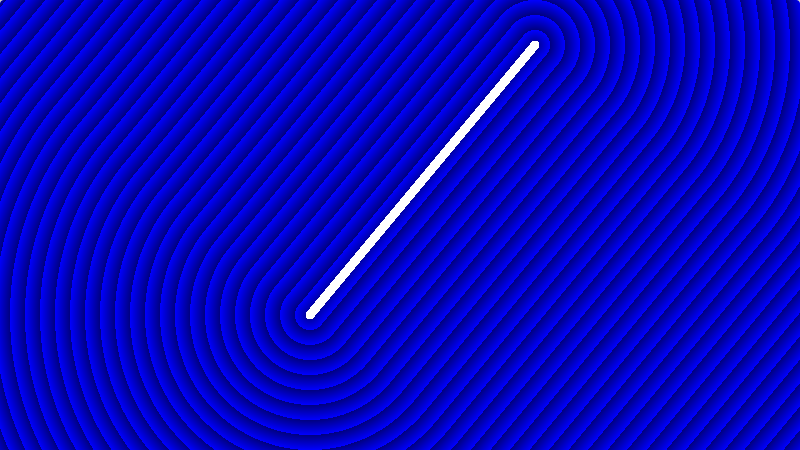
\includegraphics[width=0.8\textwidth]{secciones/imagenes/sdf/2d/sdf_segmento.png}\label{fig:segmento}
  \caption{FDS Recta que pasa por \(\Vec{a}=(-0.2, -0.2), \Vec{b}=(0.3, 0.4)\)}
\end{figure}

Existen infinitas \textit{funciones de distancia con signo exactas}, aunque muchas no han sido propuestas. Vamos, ahora, a presentar ahora algunas transformaciones u operadores que preservan su exactitud, así como otros operadores que no lo hacen y veremos su consecuencia cuando vayamos a utilizarlas para generar superficies sobre \(\mathbb{R}^3\).\\\\
Aunque no hemos podido definir más funciones, estas nociones nos ayudará a entender la definición de algunas otras funciones, por ejemplo, la definición exacta del triángulo, utiliza tres segmentos y coordenadas baricéntricas\footnote{Podemos encontrar la definición en el siguiente enlace así como la definición de este tipo de coordendas}.

\newpage

\section{Operadores sobre \(\mathbb{R}^2\)}
Vamos a ver operadores imprescindibles para poder manipular nuestra escena así como crear nuevas funciones de distancia con signo exactas.

\begin{definition}
Llamaremos \textit{Isometría} a la aplicación \(f\) entre dos espacios métricos que conservan la distancia entre los puntos. \[\forall \Vec{v},\Vec{w} \in\mathbb{R}^2, d(\Vec{v},\Vec{w})=d(f(\Vec{v}),f(\Vec{w}))\]
\end{definition}

Como estamos trabajando sobre la métrica euclídea, \(d(\Vec{v},\Vec{w})=d((x,y),(z,w))=\vert\vert \Vec{v}-\Vec{w}\vert\vert=\sqrt{(x-z)^2+(y-w)^2}\) 
Vamos a ver tres isometrías afín\footnote{Una isometría afín ...}, la tralsación, la rotación y la simetría axial. Que a partir de ahora haremos uso de aquí en adelante.

\subsection{Operador de traslación}
Dado un vector \(\Vec{t}\), definimos una traslación como el operador adición  sobre cualquier punto \(\Vec{p}\) con \(\Vec{t}\).
\[f(\Vec{p})=\text{traslacion}(\Vec{p},\Vec{t})=\Vec{p}\pm\Vec{t}\]
Vamos a demostrar que la traslación es una isometría, \(\forall \Vec{v},\Vec{w}\in\mathbb{R}^2\):
\[d(f(\Vec{v}), f(\Vec{w}))=d(\Vec{v}\pm\Vec{t}, \Vec{w}\pm\Vec{t})=\vert\vert (\Vec{v}\pm\Vec{t})-(\Vec{w}\pm\Vec{t})\vert\vert=\vert\vert \Vec{v}-\Vec{w}\vert\vert=d(\Vec{v}, \Vec{w})\]
Como se ha comentado anteriormente, las \textit{funciones de distancia con signo} han sido definidas sobre el origen, es por ello que ahora podemos trasladarnos utilizando el operador propuesto, un ejemplo sería.
\begin{lstlisting}
float escena_sdf(vec2 p){
    // Trasladamos el vector p hacia 0.1 izquierda y 0.2 a la derecha.
    vec2 pt = p - vec2(0.1, 0.2);
    return SDFCircunsferencia(pt, 0.3);
}
\end{lstlisting}

En el ejemplo anterior, hemos utilizado la resta para desplazar hacia la posición deseada, nos lo podemos imaginar como lo que en realidad movemos es el plano y no las coordenadas.

\begin{figure}[H]
  \centering
  \captionsetup{justification=centering}%,margin=2cm
  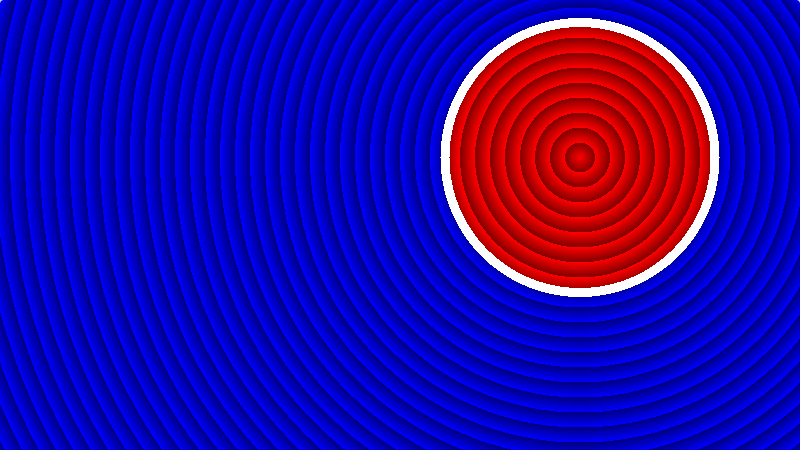
\includegraphics[width=0.8\textwidth]{secciones/imagenes/sdf/2d/sdf_traslacion.png}\label{fig:traslacion}
  \caption{Traslación FDS \(\Vec{t}=(0.1, 0.2)\)}
\end{figure}

\subsection{Operador de rotación}
Veamos como rotar una figura, esto nos puede ayudar para definir un rombo, por ejemplo. Pero antes, vamos a definir la matriz de rotación con sentido horario y ángulo \(\alpha\) en radianes:
\[ 
\text{rot}(\alpha)=\begin{pmatrix}
    +\cos(\alpha) & -\sin(\alpha)\\
    +\sin(\alpha) & +\cos(\alpha)
\end{pmatrix}
\]
que aplicada sobe un vector \(\Vec{v}=\begin{pmatrix}
    x\\
    y
\end{pmatrix}\),
\[ 
f(\Vec{p})=\text{rotacion}_\alpha(\Vec{p})=\Vec{v}\cdot\text{rot}(\alpha)=\begin{pmatrix}
    x\\
    y
\end{pmatrix}^t\cdot\begin{pmatrix}
    +\cos(\alpha) & -\sin(\alpha)\\
    +\sin(\alpha) & +\cos(\alpha)
\end{pmatrix}
\]
\[\text{rotacion}_\alpha(\Vec{p})=\begin{pmatrix}
    +x\cos(\alpha) + y\sin(\alpha)\\
    -x\sin(\alpha) + y\cos(\alpha)
\end{pmatrix}
\]
Vamos a demostrar que este operador es también una \textit{isometría}, \(\forall \Vec{v},\Vec{w}\in\mathbb{R}^2\):
\[d(f(\Vec{v}), f(\Vec{w}))=d(\Vec{v}\cdot \text{rot}(\alpha), \Vec{w}\cdot \text{rot}(\alpha))=\]\[\vert\vert \Vec{v}\cdot \text{rot}(\alpha)- \Vec{w}\cdot \text{rot}(\alpha)\vert\vert=\vert\vert(\Vec{v}-\Vec{w})\cdot \text{rot}(\alpha)\vert\vert\]
Como \(\text{rot}(\alpha)\) es ortogonal, 
\footnote{Aplicamos una propiedad de las matrices ortogonales cuya demostración se puede encontrar en el siguiente enlace https://math.stackexchange.com/questions/1754712/orthogonal-matrix-norm} \(\vert\vert A\cdot\text{rot}(\alpha)\vert\vert=\vert\vert A\vert\vert\)
\[\vert\vert(\Vec{v}-\Vec{w})\cdot \text{rot}(\alpha)\vert\vert=\vert\vert\Vec{v}-\Vec{w})\vert\vert=d(\Vec{v},\Vec{w})\]
En código,
\begin{lstlisting}
#define PI 3.1415
mat2 rot(float a){
    return mat2(
        +cos(a), -sin(a), 
        +sin(a), +cos(a)
    );
}
// Escena
float escena_sdf(vec2 p){
    // Rotacion del el vector p 45 grados o pi / 4 radianes.
    vec2 pr = p * rot(45. * PI / 180.);
    return SDFRectangulo(pr, vec2(0.3));
}
\end{lstlisting}

\begin{figure}[H]
  \centering
  \captionsetup{justification=centering}%,margin=2cm
  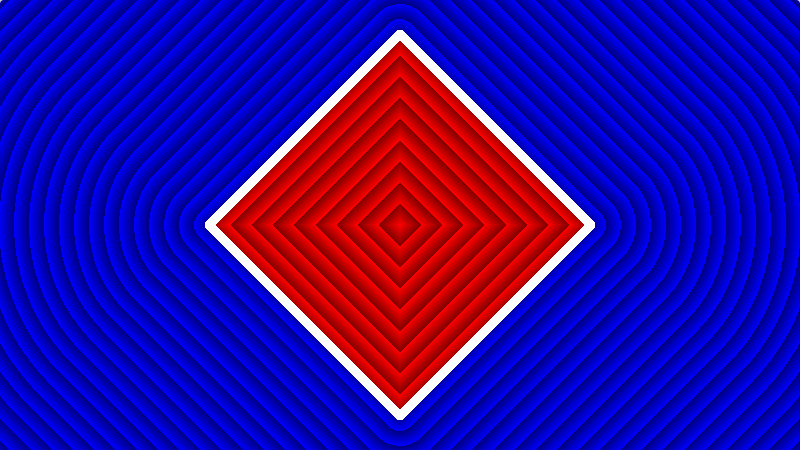
\includegraphics[width=0.8\textwidth]{secciones/imagenes/sdf/2d/sdf_rotacion.png}\label{fig:rotacion}
  \caption{Rectángulo (cuadrado) FDS con rotación \(\alpha=\dfrac{\pi}{4}\)}
\end{figure}

\subsection{Operador de simetría}
La simetría realiza un reflejo sobre una recta o alguno de los ejes, para ello, vamos a utilizar dos puntos que definen a la recta \(\Vec{a}, \Vec{b}\in\mathbb{R}^2\).
Para este cálculo, miraremos la proyección del punto \(\Vec{p}\) sobre la recta y trasladarlo hacia el otro lado de la recta sobre la dirección al punto proyectado.
\[\text{simetria}_{\Vec{a}}(\Vec{b})=2(\text{proy}_{\Vec{a}}(\Vec{b})-\Vec{b})\]
Donde \(\Vec{a}\) es un vector director de la recta que pasa por el \(0,0\). Para una recta formada por dos puntos \(\Vec{a}, \Vec{b}\), el operador de simetría será:
\[\text{simetria}_{\Vec{a},\Vec{b}}(\Vec{p}) = \text{simetria}_{\Vec{b}-\Vec{a}}(\Vec{p}-\Vec{a})+\Vec{p}\]
Existen casos particulares definidos sobre los ejes, dado un punto \(\Vec{p}=(x,y)\), definimos el operador de simetría sobre el eje x como \(\Vec{p}_x=(-x,y)\) y para el eje y, el punto simétrico \(\Vec{p}_y=(x,-y)\). Este operador será útil más adelante para optimizar cálculo de funciones de distancia con signo duplicadas.
\newpage
Veamos la definición en código,
\begin{lstlisting}
// Simetría sobre el origen
vec2 simetria(vec2 a, vec2 b){    
    return 2. * (proy(b, a) - b);
}
// Sobre cualquier recta genérica formado por dos puntos, a y b.
vec2 simetria(vec2 p, vec2 a, vec2 b){    
    return p + simetria(b - a, p - a);
}
\end{lstlisting}
Veamos el ejemplo en práctica sobre la recta definida en \fullref{fig:recta} con la función de distancia con signo definida en \fullref{fig:segmento}.
\begin{lstlisting}
float escena_sdf(vec2 p){
    // Recta Simetría
    vec2 a = vec2(0.2, 0.2);
    vec2 b = vec2(0.0, 0.1);
    // Simetría
    vec2 ps = simetria(p, a, b);
    
    return SDFSegmento(
        ps,
        vec2(-0.2, -0.2), 
        vec2(0.3, 0.4)
    );
}
\end{lstlisting}

\begin{figure}[H]
  \centering
  \captionsetup{justification=centering}%,margin=2cm
  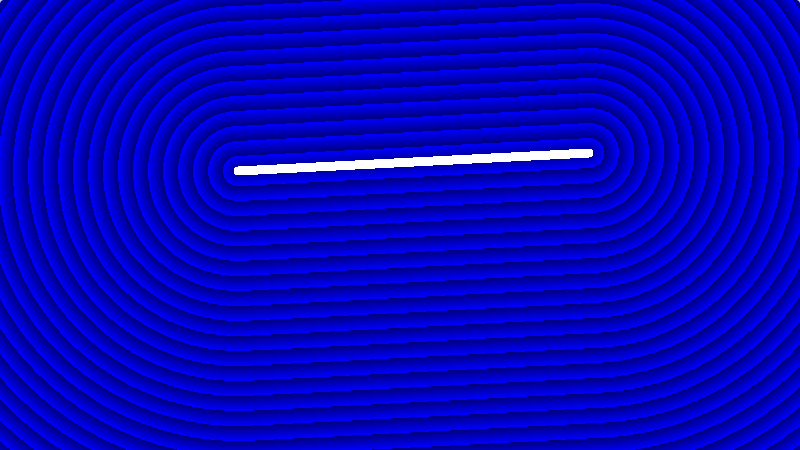
\includegraphics[width=0.8\textwidth]{secciones/imagenes/sdf/2d/sdf_simetria.png}\label{fig:simetria}
  \caption{Simetría FDS ejemplos anteriores}
\end{figure}

Veamos ahora dos operadores entre distintas \textit{funciones de distancia con signo}. Estos operadores van a ser vitales para crear escenas complejas ya que van a permitir agregar o sustraer \textit{funciones de distancia con signo exactas}.

\subsection{Operador de agregación}
Ya vista la función de traslación, ahora nos puede ser útil ver como agregar dos \textit{funciones de distancia con signo}, para así poder crear escenas más complejas. Como su propio nombre indica, si tenemos dos funciones de esta categoría, las cuales devuelven la distancia de manera individual a la superficie o perímetro más cercano, debemos quedarnos con la distancia más pequeña de las dos. Es por eso que el operador de agregación, se define como:
\[\text{Agregacion}(\Vec{p}, f, g) = \min(f(\Vec{p}), g(\Vec{p})) \]
que haremos uso de la función definida por el lenguaje \textit{GLSL}, \textit{min}. Veamos un ejemplo con dos ejemplos de \textit{isometrías}, la traslación \fullref{fig:traslacion} y la rotación \fullref{fig:rotacion}.
\begin{lstlisting}
// Escena
float escena_sdf(vec2 p){
    // Rotamos el rectángulo 45 grados - f
    vec2 pr = p * rot(PI / 180. * 45.0);
    // Trasladamos el rectangulo hacia 0.1 - g izquierda y 0.2 a la derecha.
    vec2 pt = p - vec2(0.4, 0.15);
    // Unión de dos FDS
    return min(
        SDFRectangulo(pr, vec2(0.3)), // f
        SDFCircunsferencia(pt, 0.3)   // g
    );
}
\end{lstlisting}

\begin{figure}[H]
  \centering
  \captionsetup{justification=centering}%,margin=2cm
  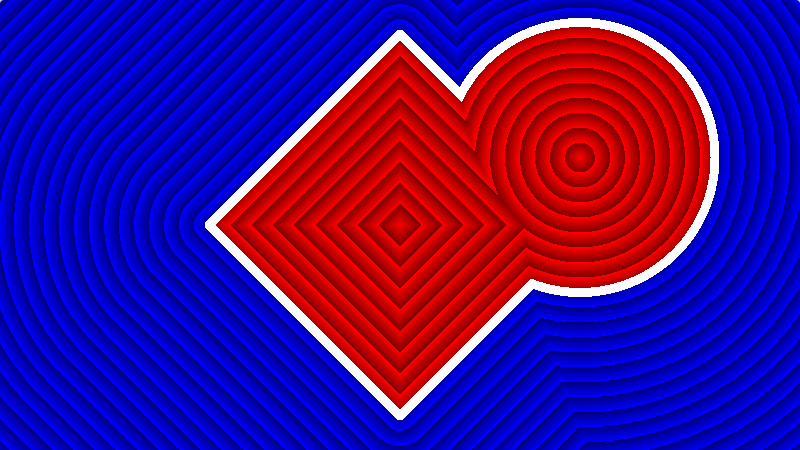
\includegraphics[width=0.8\textwidth]{secciones/imagenes/sdf/2d/sdf_add.png}\label{fig:add}
  \caption{ Adición de dos FDS de ejemplos anteriores}
\end{figure}
Se puede encadenar varias \textit{FDS} componiendo múltiples veces el operador \textit{min} sobre las distintas figuras. \\\\
Como vemos, este operador funciona como un \textit{or} en el diagrama de Venn\footnote{El diagrama de Venn}.

\subsection{Operador de substracción}
Antes hemos visto que el operador \enquote{\(\min\)} combina dos \textit{FDS}. El operador \enquote{\(\max\)} devuelve la distancia más lejana, esto quiere decir que devuelve siempre el exterior de alguna de las dos figuras en caso de existir. El interior de las figuras en caso de que ambas figuras se solapen, ya que, en caso de estar en el interior, nos quedaremos con la máxima distancia negativa.

\begin{figure}[H]
  \centering
  \captionsetup{justification=centering}%,margin=2cm
  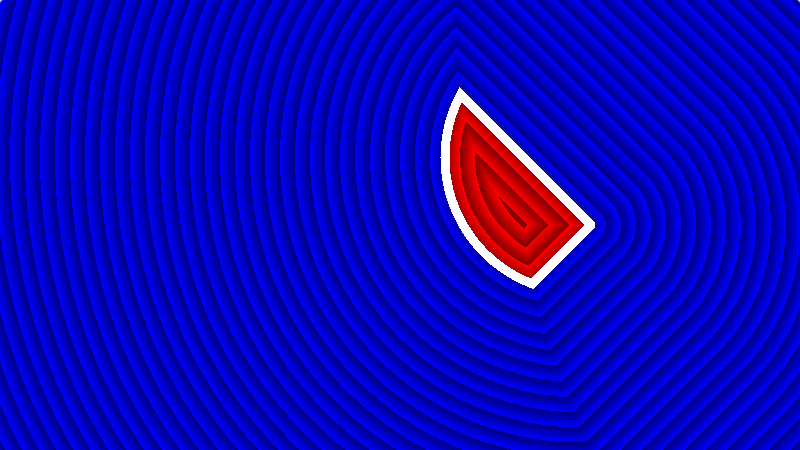
\includegraphics[width=0.8\textwidth]{secciones/imagenes/sdf/2d/sdf_subtract-1.png}\label{fig:disyunccion}
  \caption{ Disyunción de dos FDS de ejemplos anteriores}
\end{figure}

Vemos que el operador funciona como \textit{and} en el diagrama de Venn. Pero en la práctica, resulta poco útil, por lo que vamos a definir otra operación que junto a este, nos ayudará crear el operador de substracción. Podemos a cualquier \textit{función de distancia con signo} cambiar el interior por el exterior, multiplicando por \(-1\).

\begin{figure}[H]
  \centering
  \captionsetup{justification=centering}%,margin=2cm
  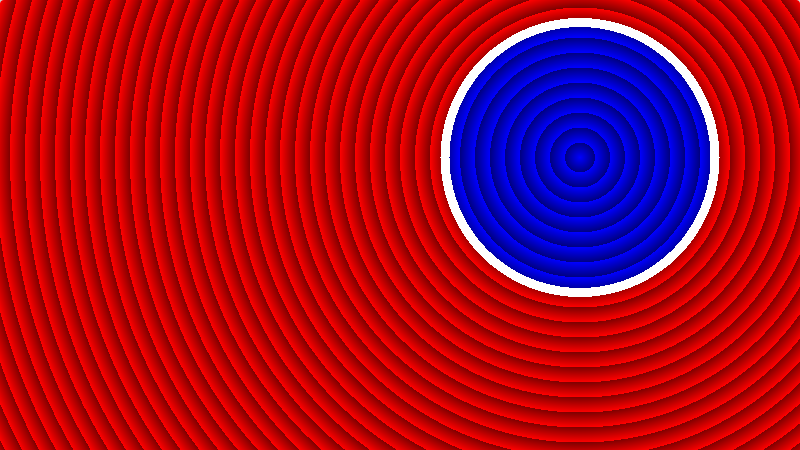
\includegraphics[width=0.8\textwidth]{secciones/imagenes/sdf/2d/sdf_subtract-2.png}\label{fig:negative}
  \caption{ Interior por Exterior Circunsferencia FDS}
\end{figure}

Viendo la imagen, observamos que las distancias negativas representan el exterior y ahora, junto con la definición dada anteriormente de substracción, aquella zona donde las distancias negativas coinciden, o mejor, aquellos puntos donde las figuras no se solapan, serán los resultantes. Podemos definir la substracción de una función de distancia con signo \(f\) otra \(g\) tal que:
\[\text{substraccion}(\Vec{p}, f,g)=max(f(\Vec{p}), -g(\Vec{p}))\]
En código,
\begin{lstlisting}
float escena_sdf(vec2 p){
    // Rotamos el rectángulo 45 grados
    vec2 pr = p * rot(PI / 180. * 45.0);
    
    // Trasladamos el rectangulo hacia 0.1 izquierda y 0.2 a la derecha.
    vec2 pt = p - vec2(0.4, 0.15);
    // Sustraemos Una circunsferencia de un rectángulo.
    return max(
        SDFRectangulo(pr, vec2(0.3)),
        -SDFCircunsferencia(pt, 0.3)
    );
}
\end{lstlisting}

\begin{figure}[H]
  \centering
  \captionsetup{justification=centering}%,margin=2cm
  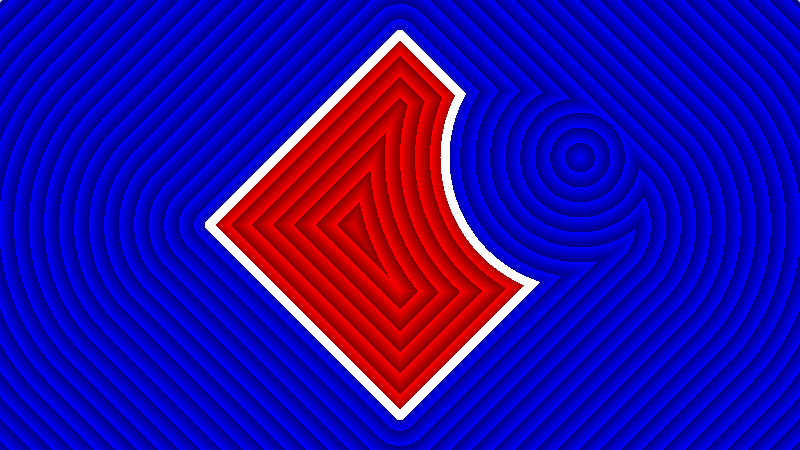
\includegraphics[width=0.8\textwidth]{secciones/imagenes/sdf/2d/sdf_subtract-3.png}\label{fig:substraction}
  \caption{Substracción de una circunsferencia a un rectangulo FDS}
\end{figure}

Cabe destacar que esta figura no preserva las distancias, por lo que el objeto restado tendrá el espacio distorsionado, veremos en los siguientes capítulos, como solucionarlo.\\\\ Vamos a ver otras transformaciones que manipulan el espacio, esto hará que estas funciones no sean exactas, pero hay situaciones en las que al no conocer la fórmula exacta, resulta más fácil manipular el espacio.

\subsection{Operador de escalado}
Veamos la deformación más sencilla y como podemos solucionar esta deformación para así no tener que manipular el \textit{Marcher}.
Supongamos que existe una isometría que reduce las distancas, es decir:
\[f(\Vec{p})=\Vec{p}\cdot \dfrac{1}{k}, k \in \mathbb{R}^{+}_{0}\]
Vemos que \(k\) es el factor de escalado, veamos que no es una isometría y como lo solucionamos, \(\Vec{v},\Vec{w}\in \mathbb{R}^2\).
\[d(f(\Vec{v}),g(\Vec{w}))=d(\Vec{v}\cdot \dfrac{1}{k}, \Vec{w}\cdot \dfrac{1}{k}) = \vert\vert \Vec{v}\cdot \dfrac{1}{k} - \Vec{w}\cdot \dfrac{1}{k}\vert\vert=\vert\vert (\Vec{v} - \Vec{w})\cdot \dfrac{1}{k}\vert\vert\]
Vemos que la distancia transformada es proporcional a la distancia inicial con factor \(k\). Para solucionar esto, multiplicamos la distancia por el factor \(k\) y consiguiendo así una isometría.
En código,

\begin{lstlisting}
// Escalado con factor k
vec2 escena_sdf(vec2 p){
    // Factor de escalado, k=0.5, mitad original. 
    float k = 0.5;
    // Escalamos
    vec2 pk = p / k; 
    // Dividimos la distancia entre el factor de escalado para conseguir una isometría.
    return primitiva(pk) * k;
}
\end{lstlisting}

La función \textit{primitiva} representa cualquier \textit{función de distancia con signo}. Si \(k<1\) estamos escalando hacia abajo, cuando \(k=1\), estamos preservando el tamaño original, finalmente, con \(k>1\) estamos escalando hacia arriba.\\\\
Veamos un ejemplo complejo, por ejemplo, escalamos el ejemplo anterior con un factor de \(k=0.5\) o la mitad:

\begin{lstlisting}
float escena_sdf(vec2 p){
    // Factor de escalado
    float k = 0.5;
    // Escalamos
    p = p / k;
    
    // Rotamos el rectángulo 45 grados
    vec2 pr = p * rot(PI / 180. * 45.0);
    // Trasladamos el rectangulo hacia 0.1 izquierda y 0.2 a la derecha.
    vec2 pt = p - vec2(0.4, 0.15);
    
    // Sustraemos Una circunsferencia de un rectángulo.
    float d = max(
        SDFRectangulo(pr, vec2(0.3)),
        -SDFCircunsferencia(pt, 0.3)
    );
    // Multiplicamos por la distancia para hacerlo una isometría.
    return d * k;
}
\end{lstlisting}

\begin{figure}[H]
  \centering
  \captionsetup{justification=centering}%,margin=2cm
  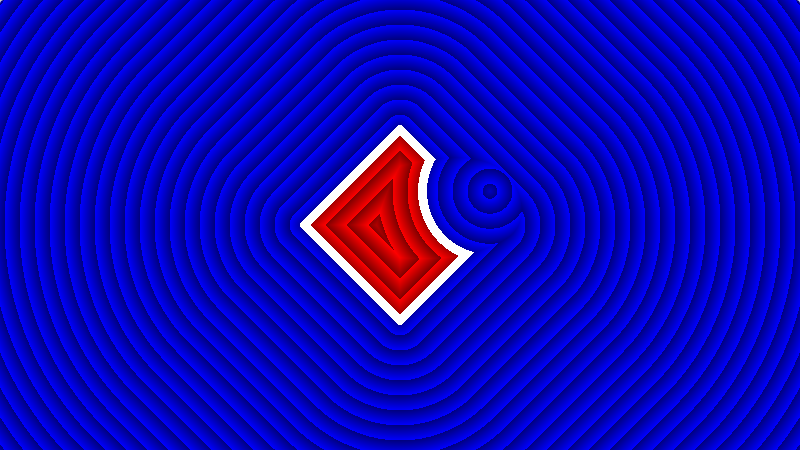
\includegraphics[width=0.8\textwidth]{secciones/imagenes/sdf/2d/sdf_subtracted_scale.png}\label{fig:substraction}
  \caption{\fullref{fig:substraction} escalado \(k=0.5\)}
\end{figure}

\subsection{Operador de deformación sin exactitud}
Eisten deformaciones que no preservan la métrica, es decir, hace que la función no sea exacta. En general, consiste en manipular el vector \(\Vec{p}\) antes de ser utilizado en nuestra función de distancia con signo, esto provocará una modificación del \textit{Marcher} cuando lo tratemos en el espacio \( \mathbb{R}^3 \) y su eficiencia.

Se trata de una aplicación \(g:\mathbb{R}^2\longrightarrow \mathbb{R}^2\) el cual no es una isometría, transformando la \textit{función de distancia con signo exacta} en otra, no exacta.
\[ \forall \Vec{x}, \Vec{y} \in \mathbb{R}^2, d(g(x), g(y)) \neq d(x,y) \]
Se recomienda utilizar aplicaciones \( g\) que sean continuas y derivables, para así evitar transformaciones fuertes. Por ejemplo,
\[g(x,y)=(x * cos(y \cdot \pi), y * sin(y \cdot \pi)\]
En código,
% TODO: Circunsferencia -> Circunferencia
\begin{lstlisting}
float sdf(vec2 p){
	// Vec2 No Isometría
	vec2 pn = vec2(
	    p.x * cos(p.y * PI),
	    p.y * sin(p.y * PI)
	);
	return SDFCircunferencia(pn, 0.1);
}
\end{lstlisting}
El resultado de la deformación:
\begin{figure}[H]
  \centering
  \captionsetup{justification=centering}%,margin=2cm
  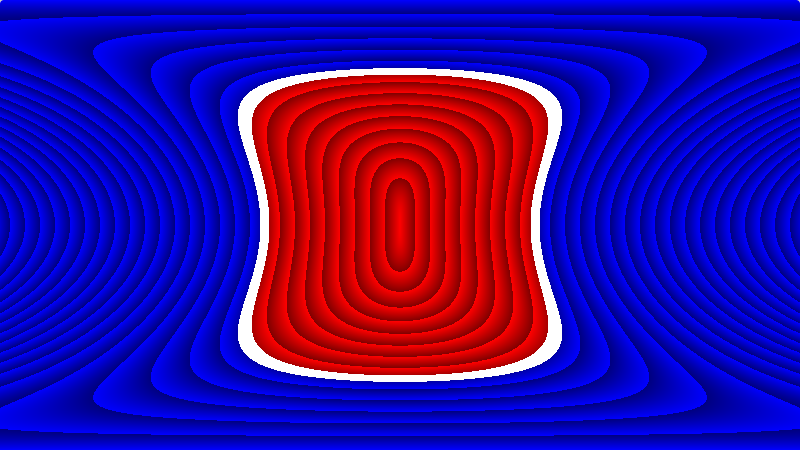
\includegraphics[width=0.8\textwidth]{secciones/imagenes/sdf/2d/sdf_deform.png}\label{fig:deform}
  \caption{Deformación del espacio de una circunsferencia FDS}
\end{figure}

Las aplicaciones explicadas anteriormente, en general, se extienden a \(\mathbb{R}^3\). Por ejemplo, vamos a ver como primitivas generalizan a las de una dimensión superior.

\section{Primitivas en \(\mathbb{R}^3\)}

\subsection{Esfera exacta}
Esta función es generalizada de la ecuación en 2D, la idea es la misma, aquellas distancias que antes eran positivas con valor \(r\), quedan anuladas al restarles \(r\) y por tanto, forman una \textit{isosuperficie}. En código,
\begin{lstlisting}
// Esfera R3
float SDFEsfera(vec3 p, float r){
    return length(p) - r;
}
\end{lstlisting}
Utilizando el \textit{Marcher} y el \textit{modelo de iluminación de Phong}, el resultado es el observado en la \fullref{fig:phong}.

\subsection{Prisma rectangular exacto}
Este generaliza de la misma forma, el valor absoluto situará las coordenadas en el cuadrante positivo, de los ocho presentes. Las medidas utilizadas serán la mitad a la original, es decir, \(\Vec{s’}= \dfrac{\Vec{s}}{2}\). Aunque no vamos a ver la demostración, una idea de esta es similar a la utilizada para demostrar el rectángulo, cada región exterior de cada cara es anulada, el interior se utiliza la distancia al lado más próximo y en la esquina, la distancia euclídea. El resultado.

\begin{lstlisting}
// Prisma R3
float SDFPrisma(vec3 p, vec3 s){
    vec3 pa = abs(p) - s;
    return length(max(pa, 0.)) +
    min(max(max(pa.x, pa.y), pa.z), 0.);
}
\end{lstlisting}

Para la visualización de este resultado, vamos a aplicar una rotación sobre el eje \(YZ\) que lo veremos para \(\mathbb{R}^3\) en la siguiente sección.

\begin{lstlisting}
float escena_sdf(vec3 p){
    // Rotacion plano yz
    vec3 pr = vec3(p.x, p.yz * rot(PI/4.0));
    // Cubo s=0.3 => s'=0.15
    vec3 sp = vec3(0.15);
    return SDFPrisma(pr, sp);
}
\end{lstlisting}

El resultado,
\begin{figure}[H]
  \centering
  \captionsetup{justification=centering}%,margin=2cm
  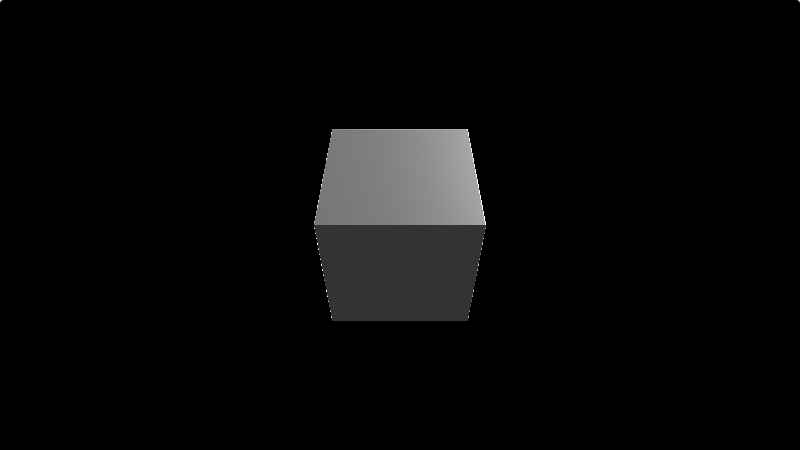
\includegraphics[width=0.8\textwidth]{secciones/imagenes/sdf/3d/sdf_prisma_rect.png}\label{fig:prisma}
  \caption{Prisma Rectangular \(\Vec{s}=\Vec{0.3}\) rotado \(\alpha_{YZ}=\dfrac{\pi}{4}\) FDS}
\end{figure}

\subsection{Plano con signo}
% TODO: Ordenar el texto de la normal.
Un plano con signo significa que dado los dos subespacios en el que se divide \(\mathbb{R}^3\), uno tendrá valores positivos y el otro, negativos. En general, los valores en los que la normal del plano tengan producto escalar negativo con el vector director de estos hacia el plano, serán positivos, para esto, definimos el operador de signo, \(\text{sign}(a)=\pm 1, 0\).\\\\
Esta función nos será muy útil junto con el operador de substracción para cortar figuras. Su demostración se basa en la proyección de un punto al plano, supondremos que el plano contiene el punto \((0,0,0)\) y tiene un vector normal \(\Vec{n}\) \footnote{Podemos definir un plano utilizando únicamente la normal de este y obligando a contener el \(\Vec{0}\)}.
\[\text{proy}_{\Vec{n}}(\Vec{p}) = \Vec{p} - (\Vec{n}\cdot\Vec{p})\Vec{n} \]
Por lo que la distancia con signo a este:
\[ SDFPlano_{\Vec{n}}(\Vec{p})=\text{sign}\left((\Vec{p}-\text{proy}_{\Vec{n}}(\Vec{p})\right) \cdot \Vec{n})\cdot \vert \vert \Vec{p} - \text{proy}_{\Vec{n}}(\Vec{p}) \vert\vert \]
Simplificamos esta ecuación,
\[ SDFPlano_{\Vec{n}}(\Vec{p}) = \text{sign}\left((\Vec{n}\cdot\Vec{p})\Vec{n}\right) \cdot \Vec{n})\cdot \vert \vert (\Vec{n}\cdot\Vec{p})\Vec{n}  \vert\vert \]
Utilizando las siguientes propiedades: \(\Vec{n}k\cdot\Vec{n}=k\) y \(\vert\vert k\Vec{n}\vert\vert=k\vert\vert\Vec{n}\vert\vert\).
\[ SDFPlano_{\Vec{n}}(\Vec{p})=\text{sign}\left(\Vec{n}\cdot\Vec{p}\right)\cdot (\Vec{n}\cdot\Vec{p}) \vert \vert\Vec{n}\vert\vert=\Vec{n}\cdot\Vec{p}\]

En código,

\begin{lstlisting}
// Plano R3
float SDFPlano(vec3 p, vec3 n){
   return dot(p, n);
}
\end{lstlisting}

Veamos un ejemplo, pero antes, vamos a desplazar el plano hacia abajo, aunque el operador de desplazamiento lo hemos visto en la sección anterior para una diension inferior, veremos que es equivalente para esta dimensión. Este desplazamiento lo tenemos que hacer ya que el plano pasa por el \((0,0,0)\), oclusionando la mitad de la pantalla.

\begin{lstlisting}
float escena_sdf(vec3 p){
    // Desplazamiento
    vec3 pt = p - vec3(0., -1., 0.);
    // Plano con normal hacia arriba
    vec3 n = normalize(vec3(0., 1., 0.));
    return SDFPlano(pt, n);
}
\end{lstlisting}

El resultado,

\begin{figure}[H]
  \centering
  \captionsetup{justification=centering}%,margin=2cm
  
\includegraphics[width=0.8\textwidth]{secciones/imagenes/sdf/3d/sdf_plano.png}\label{fig:plano}
  \caption{Plano \(\Vec{n}=(0,1,0)\) desplazado \(\Vec{t}=(0, -1, 0)\)}
\end{figure}

\subsection{Recta Exacta}

La proyección sobre una recta está definida de manera equivalente para una dimensión superior, al igual que la proyección restringinda al \([0,1]\) o el segmento.
En código,
\begin{lstlisting}
// Proyección a sobre b
vec3 proy(in vec3 a, in vec3 b){
    return b * dot(b, a) / dot(b, b);
}
// Proyección a sobre b restringido 0, 1
vec3 proy01(in vec3 a, in vec3 b){
    return b * clamp(dot(b, a) / dot(b, b), 0., 1.);
}
// Recta SDF
float SDFRecta(vec3 p, vec3 a, vec3 b){
    vec3 v = p - a;
    vec3 w = b - a;
    return length(v -  proy(v, w));
}
// Segmento SDF
float SDFSegmento(vec3 p, vec3 a, vec3 b){
    vec3 v = p - a;
    vec3 w = b - a;
    return length(v -  proy01(v, w));
}
\end{lstlisting}

\begin{figure}[H]
  \centering
  \captionsetup{justification=centering}%,margin=2cm
  \subfloat[Imagen original]{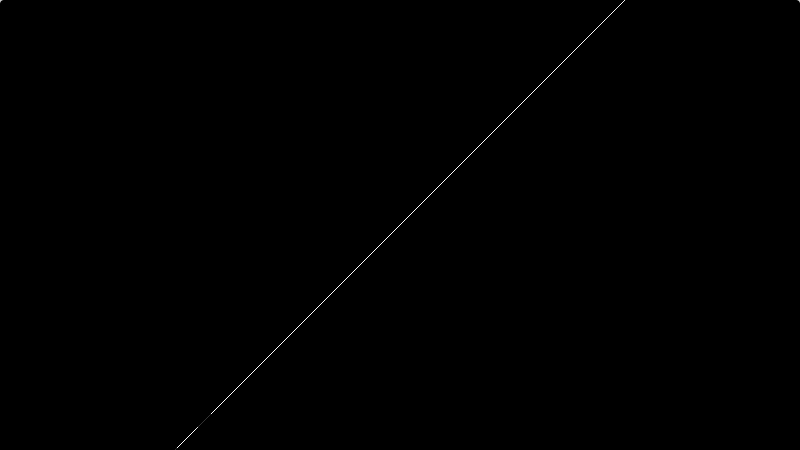
\includegraphics[width=0.4\textwidth]{secciones/imagenes/sdf/3d/sdf_recta_3d.png}\label{fig:recta3d}}
  \hfill
  \subfloat[\(f\) aplicada sobre la imagen original]{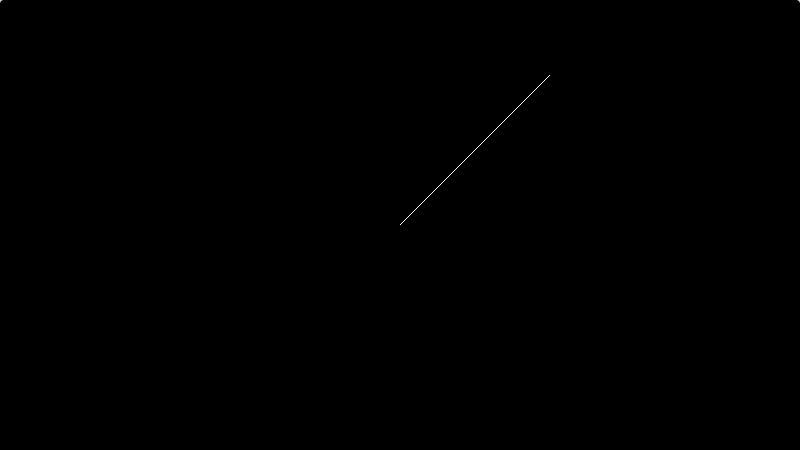
\includegraphics[width=0.4\textwidth]{secciones/imagenes/sdf/3d/sdf_segmento_3d.png}\label{fig:segmento3d}}
  \caption{Recta y Segmento Exacto \(\Vec{a}=\Vec{0}\), \(\Vec{b}=\Vec{0.5}\) SDF}
\end{figure}

Veremos un operador para incrementar el ancho de la recta o del segmento. Algunos de los operadores que vamos a ver también son generalizaciones de los operadores también  vistos en \(\mathbb{R}^2\).

\section{Operadores sobre \(\mathbb{R}^3\)}

\subsection{Operadores Isométricos}
Estos operadores son equivalentes a los \textit{Operadores sobre \(\mathbb{R}^2\)} isométricos vistos en secciones anteriores, encontramos la traslación, la rotación, la simetría y el escalado. Se puede demostrar que los operadores son isometrías de manera equivalente.\\\\
En particular, vamos a ver la rotación ya que esta se ha visto sobre el plano \(\mathbb{R}^2\) que en el espacio 3-dimensional, representa el plano \(\overline{XY}\). Definimos una rotación sobre cada uno de los tres planos como:
\[\text{rotacion}_{\overline{XY}}^\alpha(\Vec{p}) = \left(x\cos(\alpha) + y\sin(\alpha),-x\sin(\alpha) + y\cos(\alpha),z\right) \]
\[\text{rotacion}_{\overline{YZ}}^\alpha(\Vec{p}) = \left(x, y\cos(\alpha) + z\sin(\alpha),-y\sin(\alpha) + z\cos(\alpha)\right) \]
\[\text{rotacion}_{\overline{XZ}}^\alpha(\Vec{p}) = \left(x\cos(\alpha) + z\sin(\alpha),y,-x\sin(\alpha) + z\cos(\alpha)\right) \]
Aunque su definición parece bastante compleja, en código es bastante simple de implementar,
\begin{lstlisting}
// Matriz de Rotacion
mat2 rot(float a){
    return mat2(
        +cos(a), -sin(a), 
        +sin(a), +cos(a)
    );
}
// Rotación del plano XY
vec3 rotXY(vec3 p, float a){
    vec2 pr = p.xy * rot(a);
    return vec3(pr.x, pr.y, p.z);
}
// Rotación del plano YZ
vec3 rotYZ(vec3 p, float a){
    vec2 pr = p.yz * rot(a);
    return vec3(p.x, pr.x, pr.y);
}
// Rotación del plano XZ
vec3 rotXZ(vec3 p, float a){
    vec2 pr = p.xz * rot(a);
    return vec3(pr.x, p.y, pr.y);
}
\end{lstlisting}

El resultado de rotar una cubo sobre el plano \(\overline{YZ}\) lo podemos ver en la \fullref{fig:prisma}, con un ángulo \(\alpha=\dfrac{\pi}{4}\).\\\\
Vamos a ver ahora operadores que transforman figuras exactas sobre \(\mathbb{R}^2\) en otras en \(\mathbb{R}^3\) de manera exacta. Esto nos será muy útil ya que en algunos casos, calcular la \textit{función de distancia con signo exacta} en \(\mathbb{R}^2\) es más sencillo y utilizar alguno de estos operadores, puede ser de gran ayuda. Vamos a ver dos, el operador de \textit{revoloución} y \textit{extrusión}.

\subsection{Operador de ensanchamiento}
Presentamos el operador de engrosamiento, este operador va a crear otras funciones de distancia con signo con mayor superficie.\\\\
Existen figuras las cuales el marcher no es capaz de trazarlos debido a la poca superficie.\\\\  Restaremos un valor \(k\in\mathbb{R}\) a la función de distancia con signo, algunos autores \footnote{Inigo Quilez lo llama salto de isonivel https://www.iquilezles.org/www/articles/distfunctions/distfunctions.htm} llaman a la resta \enquote{salto de \textit{isosuperficie}}, aunque también se puede utilizar para \textit{isoperímetros}.\\\\ Una idea de la demostración es observar que sobre cualquier punto de una isosuperficie se puede posicionar una esfera cuya superficie es proporcional al radio, la resta de \(k\) sobre las distancias provoca un incremento del radio de la esfera y por tanto, de la superficie.  
\[\text{ensanchar}_k(\Vec{p}, f)=f(\Vec{p})-k\]
Veamos el ensanchamiento del segmento visto en \fullref{fig:segmento3d}, esta nueva función es llamada cápsula.
\begin{lstlisting}
// FDS Cápsula
float SDFCapsula(vec3 p, vec3 a, vec3 b, float k){
	return SDFSegmento(p, a, b) - k;
}
\end{lstlisting}
El resultado es el siguiente,
\begin{figure}[H]
  \centering
  \captionsetup{justification=centering}%,margin=2cm
  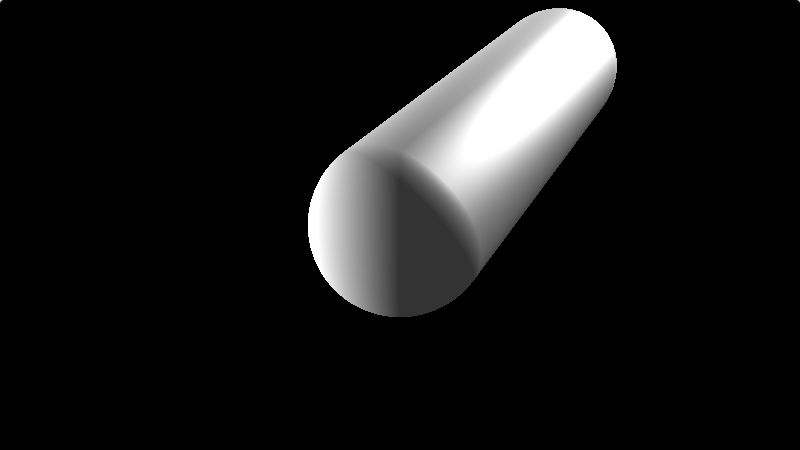
\includegraphics[width=0.8\textwidth]{secciones/imagenes/sdf/3d/sdf_capsula.png}\label{fig:capsula}
  \caption{Segmento ensanchado exacto FDS}
\end{figure}

Podemos observar que este operador devuelve una figura ensanchada con los bordes redondeados, debido a la métrica. Podemos conseguir una figura con bordes redondeados y con el tamaño original, sin ensanchar, combinándolo con el operador de escalado.

\subsection{Operador de revolución}
El primer operador es muy importante ya que nos va a permitir generar más funciones exactas utilizando las \textit{funciones de distancia con signo} de una dimensión inferior. El resultado de este operador es una figura generada por el giro sobre un eje de la figura plana.\\\\
Calculamos  

Vamos a calcular la distancia positiva al isoperímetro, dado el plano \(\overline{AB}\) sobre el que está la figura \(f:\mathbb{R}^2\longrightarrow\mathbb{R}\) y dado un punto \(\Vec{p}\in\mathbb{R}^3\) sobre la escena, la proyección de \(\Vec{p}\) sobre el plano \(\overline{AB}\) será \(\Vec{p}_{a,b}\) con \(c\) como coordenada independiente y cuya distancia de la proyección al isoperímetro será \(f(\Vec{p}_{a,b})\), por definición. Si \(\Delta h=(c-0)\) es la altura respecto de \(\Vec{p}\) sobre el plano \(\overline{AB}\), se crea un triángulo equilátero de lados \(\Delta h\) y \( f(\Vec{a,b})\) (Obsérvese la figura \fullref{fig:proof_rev}) y la distancia \Vec{p} hasta el isperímetro de la figura sobre el plano será la diagonal del triángulo formado.
\[\text{distancia}_{\overline{AB}}(\Vec{p}, f)= \sqrt{(\Delta h)^2+(f(\Vec{p}_{a,b}))^2}=\vert\vert(c, f(\Vec{p}_{a,b})\vert\vert\]

Podemos utilizar esta técnica para ensanchar también el isoperímetro trazado para la revolución:

\[\text{revolucion}_{\overline{AB}}^k(\Vec{p}, f)=\text{distancia}_{\overline{AB}}(\Vec{p}, f)-k\]

Veamos un ejemplo de una figura exacta que podemos generar, por ejemplo, un toro\footnote{Se trata de una figura en forma de donut}. La obtenemos de revolucionar una circunsferencia desplazada. En código,

\begin{lstlisting}
/// FDS Toro
float SDFToro(vec3 p, float r1, float r2){
    // FDS Circunsferencia desplazada izq r1 del centro.
    float d = length(p.xz) - r1;
    // Calculamos altura
    float dh = p.y - 0.;
    // Calculamos la distancia (la diagonal)
    return SDFCircunferencia(vec2(dh, d),r2);
}
\end{lstlisting}

\subsection{Operador de extrusión}
Este es el último operador y consiste en elongar una figura plana hacia un eje. Pudiendo ser finita o infinita. Cada punto \(\Vec{p}\in\mathbb{R}^3\) se proyecta sobre el plano a extruir y se calcula la función de distancia \(\mathbb{R}^2\). La proyección sobre los planos que conforman los ejes se calcula de manera trivial anulando la componente que no pertenece al plano. Sea \(f:\mathbb{R}^2\longrightarrow\mathbb{R}^2\) una \textit{función de distancia con signo}, una extrusión sobre el eje \(\overline{Y}\) será:
\[\text{extrusion}^\infty_{\overline{XZ}}\left(\Vec{p},f\right) = f\left(\Vec{p}_{x,z}\right)=f\left(\Vec{p}_{x}, \Vec{p}_{z}\right)\]
Dado cualquier plano \(\overline{AB}\),
\[\text{extrusion}^\infty_{\overline{AB}}\left(\Vec{p},f\right) = f\left(\Vec{p}_{a,b}\right)=f\left(\Vec{p}_{a}, \Vec{p}_{b}\right)\]
Si la extrusión quisiéramos que fuera finita, de longitud \(h\), podemos utilizar la componente independiente como longitud, esto creará una función exacta con tapadera. Utilizamos la simetría sobre el eje \(\Vec{C}\), haciendo \(h'=\dfrac{h}{2}\). La altura respecto de la tapadera con signo para cualquier punto \(\Vec{p} \in\mathbb{R}^3\) será,
\[\Delta c  =\vert\Vec{p}_c\vert - h'\]
Dividimos el ejercicio en dos subproblemas, por encima de la tapa \(\Delta c \ge 0\) y aquellas por debajo \(\Delta < 0\). Utilizaremos de referencia \fullref{fig:proof2}.

\begin{figure}[H]
  \centering
  \captionsetup{justification=centering}%,margin=2cm
  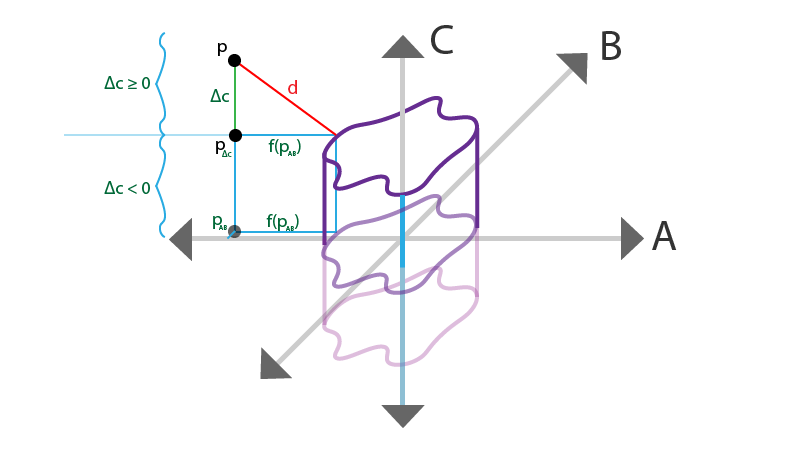
\includegraphics[width=1.0\textwidth]{secciones/imagenes/sdf/proofs/proof_extrussion.png}\label{fig:capsula}
  \caption{Visualización de una extrusión genérica}
\end{figure}

\begin{enumerate}
    \item \textbf{Subproblema 1}. La distancia puede ser negativa o positiva y corresponde con la distancia que devuelve nuesta función \(f\) sobre la proyección del punto en el plano \(\overline{AB}\).
    \[d_1=f(\text{proy}_{\overline{AB}}(\Vec{p}))=f(\Vec{p}_{a,b})\]
    \item \textbf{Subproblema 2}. Se trata de distancias positivas, observamos en la imagen que se forma un triángulo rectángulo de altura \(\Delta c\) y de base \(f(\Vec{p}_{a,b})\) equivalente al \textbf{Subproblema 1}. La diagonal \(d\) corresponde a la distancia de \(\Vec{p}\) a la superficie de la tapadera.
    \[d_2=\sqrt{(\Delta c)^2+f(\Vec{p}_{a,b})^2}\]
\end{enumerate}

Veamos como podemos unificar ambos subroblemas como hicimos con el rectángulo. Cuando \(\Delta c < 0\), queremos que \(d_1=d_2\), esto se consigue haciendo que \(\Delta c\) sea 0 cuando este sea negativo,
\[d_2=\sqrt{\max(\Delta c, 0)^2+f(\Vec{p}_{a,b})^2}=\vert\vert (\max(\Delta c, 0), f(\Vec{p}_{a,b}))\vert\vert\]

Vamos a generar el interior y exterior de la figura, los cuales se anularán de manera individual. Anularemos \(d_2\) cuando el punto esté en el interior. Para ello, en la ecuación, \(d_1\) debe anularse cuando este sea negativo.
\[d_{exterior}=\vert\vert \max((\Delta c, f(\Vec{p}_{a,b})), 0)\vert\vert\]

El interior de la figura ocurre cuando \(\Delta c < 0\) y \(d_1 < 0\), por lo que se anularán cuando sean positivos. Tomaremos el máximo de las dos distancias para encontrar la mínima negativa.
\[d_{ext} = \text{argmax}(\Delta c, d_1) = \min(\max(\Delta c, f(\Vec{p}_{a,b})), 0)\]
Finalmente, como se anulan, podemos sumar y la ecuación resultante será:
\[\text{extrusion}^h_{\overline{AB},\Vec{C}}\left(\Vec{p},f\right)=\vert\vert \max((\Delta c, f(\Vec{p}_{a,b})), 0)\vert\vert +  \text{argmax}(\Delta c, f(\Vec{p}_{a,b}))) \]

Un ejemplo de esta técnica es la fabricación del cilindro exacto con y sin tapa de radio \(r\). Los cilindros en código:
\begin{lstlisting}
// FDS circunsferencia
float SDFCircunferencia(vec2 p, float r){
	return length(p) - r;
}
/// FDS Cilindro Inifinito (Sin Tapa)
float SDFCilindroInfinito(vec3 p, float r){
    // Extrusión infinito de un cilindro sobre el plano YZ.
    return SDFCircunferencia(p.yz, r);
}
/// FDS Cilindro Finito (Con Tapa)
float SDFCilindro(vec3 p, float h, float r){
    // Extrusión de un cilindro sobre el plano YZ.
    // Altura sobre la tapa.
    float dc = abs(p.x) - h;
    // FDS Circunferencia de radio r
    float fp = SDFCircunferencia(p.yz, r);
    // Exterior figura
    float dint = length(max(vec2(dc,fp),0.));
    // Interior de la figura
    float dext = min(max(dc, fp), 0.);
    // Sumamos ambos
    return dint + dext;
}
\end{lstlisting}

Los resultados de las funciones con y sin tapa:

\begin{figure}[H]
  \centering
  \captionsetup{justification=centering}%,margin=2cm
  \subfloat[Cilindro sin tapa]{
\includegraphics[width=0.4\textwidth]{secciones/imagenes/sdf/3d/sdf_cilindro_infinito.png}\label{fig:cilindro_inf}}
  \hfill
  \subfloat[Cilindro con tapa]{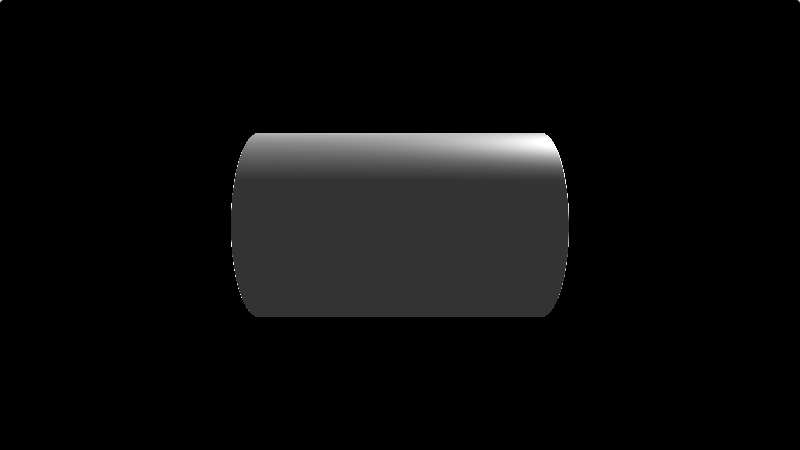
\includegraphics[width=0.4\textwidth]{secciones/imagenes/sdf/3d/sdf_cilindro.png}\label{fig:cilindro_tapa}}
  \caption{Cilindro con \(r=0.2\) y \(h'=0.3\)  FDS}
\end{figure}

\subsection{Operador de agregación y substracción}
Vamos a recordar los operadores de agregación y substracción presentados anteriormente en la sección de operadores en \(\mathbb{R}^2\). Ambos operadores tienen la misma definición, por lo que vamos a ver un ejemplo de ambos. Para ello, vamos a utilizar dos esferas con el mismo radio y una separada de la otra, como si tratara de un \textit{diagrama de Venn}.
\begin{lstlisting}
float escena_sdf(vec3 p){
    // Dos esferas, una trasladadas
    // Agregacion
    return min(
        SDFEsfera(p, 0.3),
        SDFEsfera(p - vec3(0.3, 0., 0.), 0.3)
    );
}
\end{lstlisting}
El resultado de la agregación:
\begin{figure}[H]
  \centering
  \captionsetup{justification=centering}%,margin=2cm
  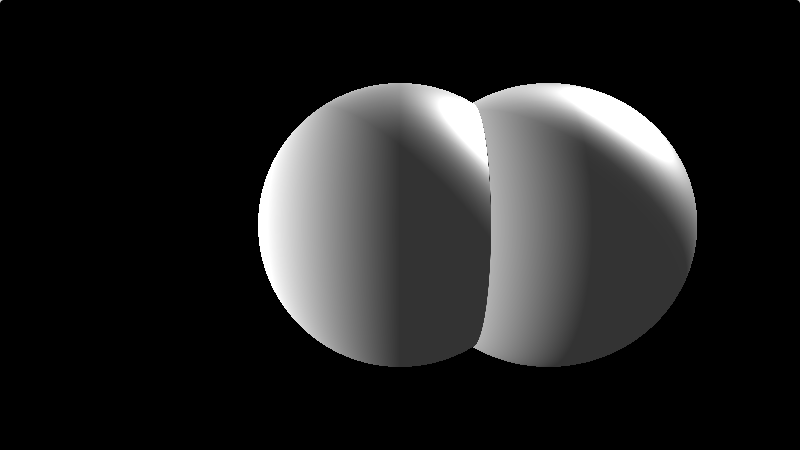
\includegraphics[width=0.8\textwidth]{secciones/imagenes/sdf/3d/sdf_add_3d.png}\label{fig:add3d}
  \caption{Agregación de dos esferas \(r=0.3\) y una trasladada}
\end{figure}

Como ya se ha comentado, el operador \enquote{\(\max\)} devuelve la intersección de ambas figuras. Vamos a utilizar la definición del plano con signo para seccionar una figura, ya que una región es sólida y la otra no. \\\\
Rotaremos la escena, utilizaremos el operador de rotación del plano \(\overline{XZ}\) con \(\alpha=\dfrac{\pi}{4}\) y poder ver así el interior:

\begin{lstlisting}
float escena_sdf(vec3 p){
    // Rotamos el plano XZ, pi / 4 rad
    p = rotXZ(p, PI / 2. * 1.2);
	// Sección de una esfera
    return max(
        SDFEsfera(p, 0.3),
        SDFPlano(p - vec3(0., 0., 0.15), vec3(0., 0., 1.))
    );
}
\end{lstlisting}

Se trata de una sección del eje \(\Vec{z}\), además, se ha aplicado el operador de traslación al plano \(\Vec{t}=(0,0,0.3)\), pudiendo así modificar la posición de la sección. El resultado es el siguiente:

\begin{figure}[H]
  \centering
  \captionsetup{justification=centering}%,margin=2cm
  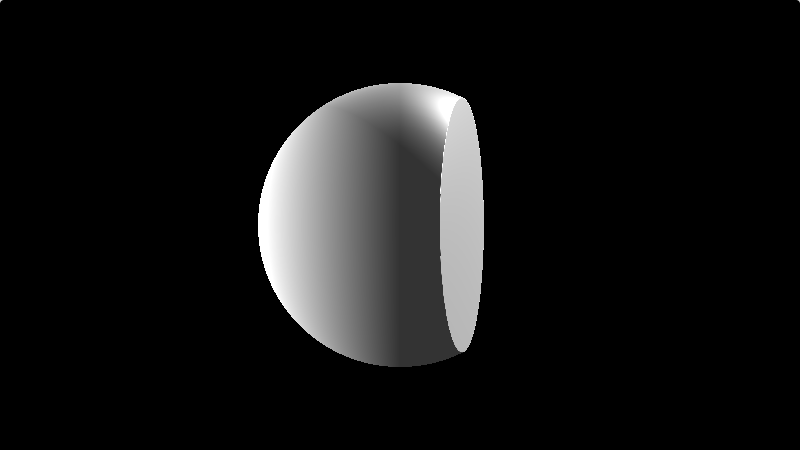
\includegraphics[width=0.8\textwidth]{secciones/imagenes/sdf/3d/sdf_seccion_3d.png}\label{fig:seccion}
  \caption{Una esfera \(r=0.3\) seccionada por un plano \(\Vec{n}=(0,0,-1)\) desplazado}
\end{figure}

En el ejemplo anterior hemos visto que el operador \enquote{\(\max\)} tiene una mayor utilidad por si solo. Vamos a presentar ahora este mismo operador pero como lo hemos visto en \fullref{fig:substraction}, vamos a cambiar el interior por el exterior de la figura a substraer, recibiendo el nombre de \enquote{carvado}. En código:

\begin{lstlisting}
float escena_sdf(vec3 p){
    // Rotamos el plano XZ, pi / 4 rad
    p = rotXZ(p, PI / 4.);
    // Dos esferas, una trasladadas
    // Substraccion b en a => max(a, -b)
    return max(
        SDFEsfera(p, 0.3),
        -SDFEsfera(p - vec3(0.3, 0., 0.), 0.3)
    );
}
\end{lstlisting}

El resultado será una esfera en el centro a la que se le ha carvado otra esfera, trasladada. El resultado:

\begin{figure}[H]
  \centering
  \captionsetup{justification=centering}%,margin=2cm
  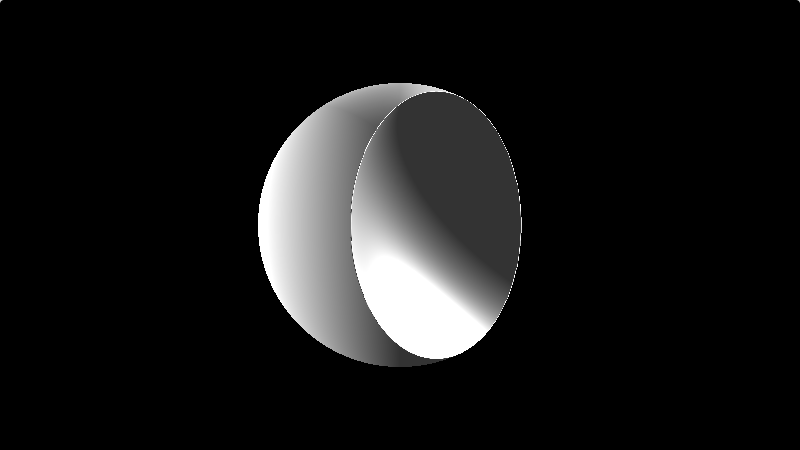
\includegraphics[width=0.8\textwidth]{secciones/imagenes/sdf/3d/sdf_substract_3d.png}\label{fig:sub3d}
  \caption{Dos esferas \(r=0.3\) y substracción de la trasladada}
\end{figure}

Este último operador no devuelve una función exacta, veamos por qué:

\subsection{Operador de deformación no exacta}

Veamos el último operador, recordemos que este no conserva la métrica, provocando lo que llamaremos \enquote{artefactos} y que veremos en el siguiente capítulo como solventarlos. Vamos a aplicar la siguiente deformación:
\[g(\Vec{p})=(
\Vec{p}_x \cos(10\Vec{p}_y) + \Vec{p}_z\sin(10\Vec{p}_y),
\Vec{p}_y,
\Vec{p}_x\sin(10\Vec{p}_y) + \Vec{p}_z\cos(10\Vec{p}_y)
)
\]
Esta deformación es conocida como \textit{torsión}, consiste en rotar un eje a medida que se incrementa la distancia a este. Utilizaremos un cubo para este ejemplo, en código:

\begin{lstlisting}
float escena_sdf(vec3 p){
    // Rotamos la escena
    vec2 ry = p.yz * rot(PI / 4.0);
    p = vec3(p.x, ry.x, ry.y);
    // Deformación "g"
    float k = 10.0; // periodo.
    float a = p.y * k;
    p = vec3(
    	+p.x * cos(a) + p.z * sin(a),
    	+p.y,
        -p.x * sin(a) + p.z * cos(a)
    );
	// Dibujamos un prisma.
    return SDFPrisma(p, vec3(0.2));
}
\end{lstlisting}

El resultado obtenido es el siguiente:

\begin{figure}[H]
  \centering
  \captionsetup{justification=centering}%,margin=2cm
  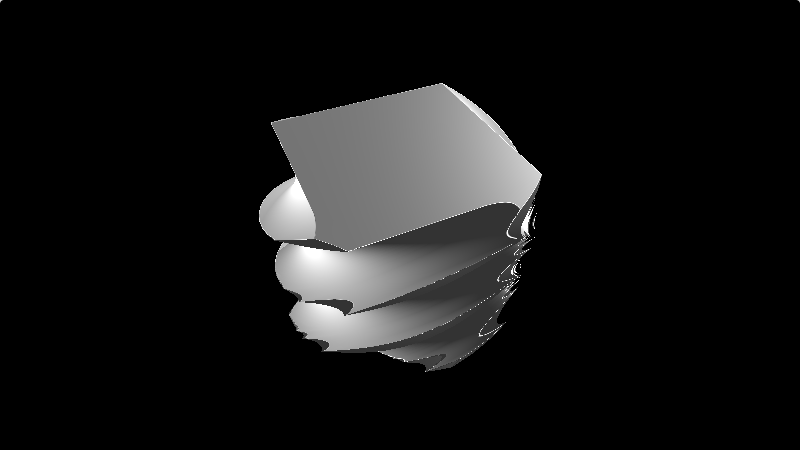
\includegraphics[width=0.8\textwidth]{secciones/imagenes/sdf/3d/sdf_twist.png}\label{fig:twist}
  \caption{Deformación torsión de un cubo \(\Vec{l}=\Vec{0.2}\)}
\end{figure}

Vemos que el resultado no es el esperado, por ejemplo, la tapadera es no es correcta en el lado inferior, vemos que este se ha deformado, el cual llamaremos \textit{artefacto}. En la siguiente sección vamos a presentar técnicas para solucionar estos problemas, aunque sean costosas.